\documentclass[a4paper,11pt]{article}

\usepackage[affil-it]{authblk}
%\usepackage{amsfonts, amsmath, amssymb, bm}
%\usepackage{float}
\usepackage[margin=1.0in]{geometry}
\usepackage{graphicx}
%\usepackage{hyperref}
%\usepackage{subcaption}
%\usepackage{subfigure}
\usepackage{url}

%\graphicspath{{../pdf/}{../jpeg/}}
% \DeclareGraphicsExtensions{.pdf,.jpeg,.png}
\graphicspath{{figures/}}

%\newcommand{\bfnull}{\textbf{null}}

\begin{document}

\title{Towards the Planning of World Domination}
\author{Jason Gregory and Kamruzzaman Quddus \\ \{jgregory, kquddus\}@umd.edu}
\affil{University of Maryland, College Park, MD}
\date{\today}

\maketitle

%
\abstract{Abstract goes here.}

\section{Introduction}\label{sec:intro}
High-level overview of topic and introduction of problem statement: Warlight AI Challenge 2.

\subsection{Problem Statement}\label{sec:problem}
Seeking to develop a robust planner for the Warlight AI Challenge 2 \cite{warlight}.
Describe rules of Warlight game (our bot vs one opponent, random map, fog of war, standard scoring and troop allocation, no cards).

\subsection{Previous Work}\label{sec:previous}
Reference other bots in challenge, publications on risk strategies, etc.

\subsection{Importance and Relevancy}\label{sec:importance}
What remains - Own implementation of planning algorithm using topics covered in this class.
Why interesting - Demonstrate topics from class in real-world example.
What is significance - Application of theoretical concepts to interesting game (and world domination)

%
\section{Technical Approach}\label{sec:approach}
High-level description of approach.

\subsection{Hypothesis}\label{sec:hypothesis}
We think a Refinement Acting Engine (RAE), SeRPE, or HTN (not sure which) will fit well into this structure and application.

\subsection{Process}\label{sec:process}
Our goal is to write the best possible AI agent algorithm for RISK game. In addition of the attributes of the classic RISK game, one of the constraints “fog of war” adds yet another dimension to the probabilistic nature of the game. The game is actually a platform of competing AI algorithms (written by other AI enthusiasts), thus the goal is to write more well thought, comprehensive and yet faster algorithm than other entrees.

Few constraints imposed by the game itself and by the game engine are : fog of war, time-limit of 500ms each turn, troop concentration can attack one region at most per turn and after each attack or transfer at least 1 troop must be left behind each region of origin. Due to the imposed constraints of the engine, any successful AI agent must successfully address the balance between run time speed vs algorithmic analysis completeness as well as resolving exploration-exploitation nature of the RISK game. Because the game itself is elementally adversarial with a lot of demanding sub components; we have decided to take hybrid approach between MAXMINI , UCT & domain specific algorithm within a hierarchical planning framework.

The general strategy for the proxy AI agent is to acquire regions in manner by which it gets stronger while being tactically flexible enough to starve the opponent from in-game advantages. Such planner needs to be adversarial in nature, hierarchical in construction, efficient and robust enough to survive game’s built-in rule and constraints. At the very high level, we believe an implantation of MAXMINI algorithm is a good candidate.

We believe the task is essentially a large state-space problem that will involve making Markovian decisions. Naturally a Monte-Carlo based approach was considered initially but due to lack of full visibility of the state space, the UCT is preferred over vanilla Monte-Carlo for low level planning & simulation.

||| Shameless Copy ||| We plan to incorporate the UCT algorithm as an initial starting point for a planner. We think this will work well because of the time constraint. We plan to evaluate our implementation, first ignoring the time constraint so that we can confirm correctness and evaluate performance. At latter stage after characterizing the performance of the algorithm, we plan to make modifications such that the planner performs well with the addition of the timer constraint. As of right now, these modifications include the notion of zones (cluster of regions) for more efficient simulation generation and the MAXMINI algorithm for enhance evaluation of individual simulation instances. We will simulate several different approaches that incorporate different modifications and compare the performance for each variant based on the number of games won as well as the required rate to win a game (in other words rounds needed divided by total rounds).

If runtime becomes an issue then further modification to the approach may involve : prioritized actions, re-prioritized events, constant depth for UCT tree generation e.t.c. These details will be explored during development and debugging stage.

The look ahead of possible actions are performed by UCT to a level of depth allowed by time-constraint. Intuitively optimal solution due to game constraint (ex: fog of war) is thought to be unachievable. The motivation is to create near-optimal solution.

Any domain specific algorithm mixed within this hybrid approach will be a purely algorithmic translation of the author’s bias towards particular preferred style of playing this game

Essential elements such as parsing routines as sensor/actuator platform will generate commands for the engine, events, create/update sate variables and possibly some book-keeping resources such as look-up tables (to be used by probabilistic routines) will also need to be developed. State variables, tasks and events will work as the  communication scheme between each level of this hierarchical adversarial planner.

Hypothetically the proposed approach could produce mixed result and is subjected to: size of map, competence of opponent’s algorithm. The final approach and detailed mechanism is subjected to change. The effectiveness of the proposed algorithm will be bench marked and ranked by other competing algorithms also submitted for the same gaming platform.


%
\section{Project Management}\label{sec:management}
The main tasks of this project include implementing the UCT algorithm, conducting simulations, and evaluating the generated data so that we can publish our results in a report and a presentation. 

\subsection{Tasks}\label{sec:tasks}
There are seven main tasks required to successfully develop a planner that is capable of winning a game in the Warlight AI Challenge 2.  The first, which we have already completed, is a literature review of the UCT algorithm, its variants, and its application to the planning of games involving artificial intelligence. The next task is formulating the problem in a manner that is compatible with our proposed approach. With a concrete understanding for a possible solution, the next task is to implement the basic UCT algorithm.  The next two tasks consist of testing, modifying and improving our implementation to enhance the performance of our solution.  A simulation and evaluation of our algorithm is required to determine how well it performs compared to other strategies. Finally, we will present our results in a report and a presentation.  These tasks, with their respective tentative deadlines and durations are summarized in Table~\ref{tab:deadlines} and Figure 1. %~\ref{fig:gantt}.

%
\begin{table}[tbp]
  \centering
  \begin{tabular}{|c|c|}
    \hline
    \emph{Task} & \emph{Deadline} \\ 
    \hline
    Literature Review & March 9, 2015 \\ \hline
    Problem Formulation & March 16, 2015 \\ \hline
    UCT Implementation & April 6, 2015 \\ \hline
    Testing & April 13, 2015 \\ \hline
    UCT Modification and Improvement & April 13, 2015 \\ \hline
    Simulation and Evaluation & April 27, 2015 \\ \hline
    Write Report and Presentation & May 2, 2015 \\ \hline
  \end{tabular}
  \caption{Table of deadlines.}
  \label{tab:deadlines}
\end{table}

%
\begin{figure}[tbp]
  \centering
  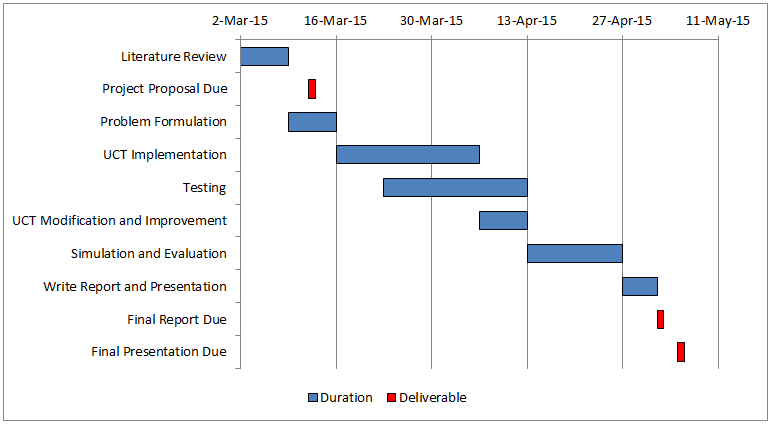
\includegraphics[width=0.95\columnwidth]{gantt_chart}
  \label{fig:gantt}
  \caption{Gantt chart}
\end{figure}

\subsection{Assignments}\label{sec:assignments}
Divide and conquer tasks, WAR code, etc.

\subsection{Schedule}\label{sec:schedule}
Gantt chart with milestones and dates.

%
\section{Conclusions}\label{sec:conclusions}
Summary of problem and intended approach.

% References 
\bibliographystyle{plain}
\bibliography{references}

% End document
\end{document}

